\section{Analysis of Clocked Sequential Circuits}
\label{sec:analysis-clocked-seq-circ}

\subsection{State Equations}
\label{subsec:state-equations}

A \textit{state equation} (also called a \textit{transition equation}) specifies the next state as a function of the present state and inputs. Consider the sequential circuit shown in Fig. 15
\begin{figure}[H]
  \centering
  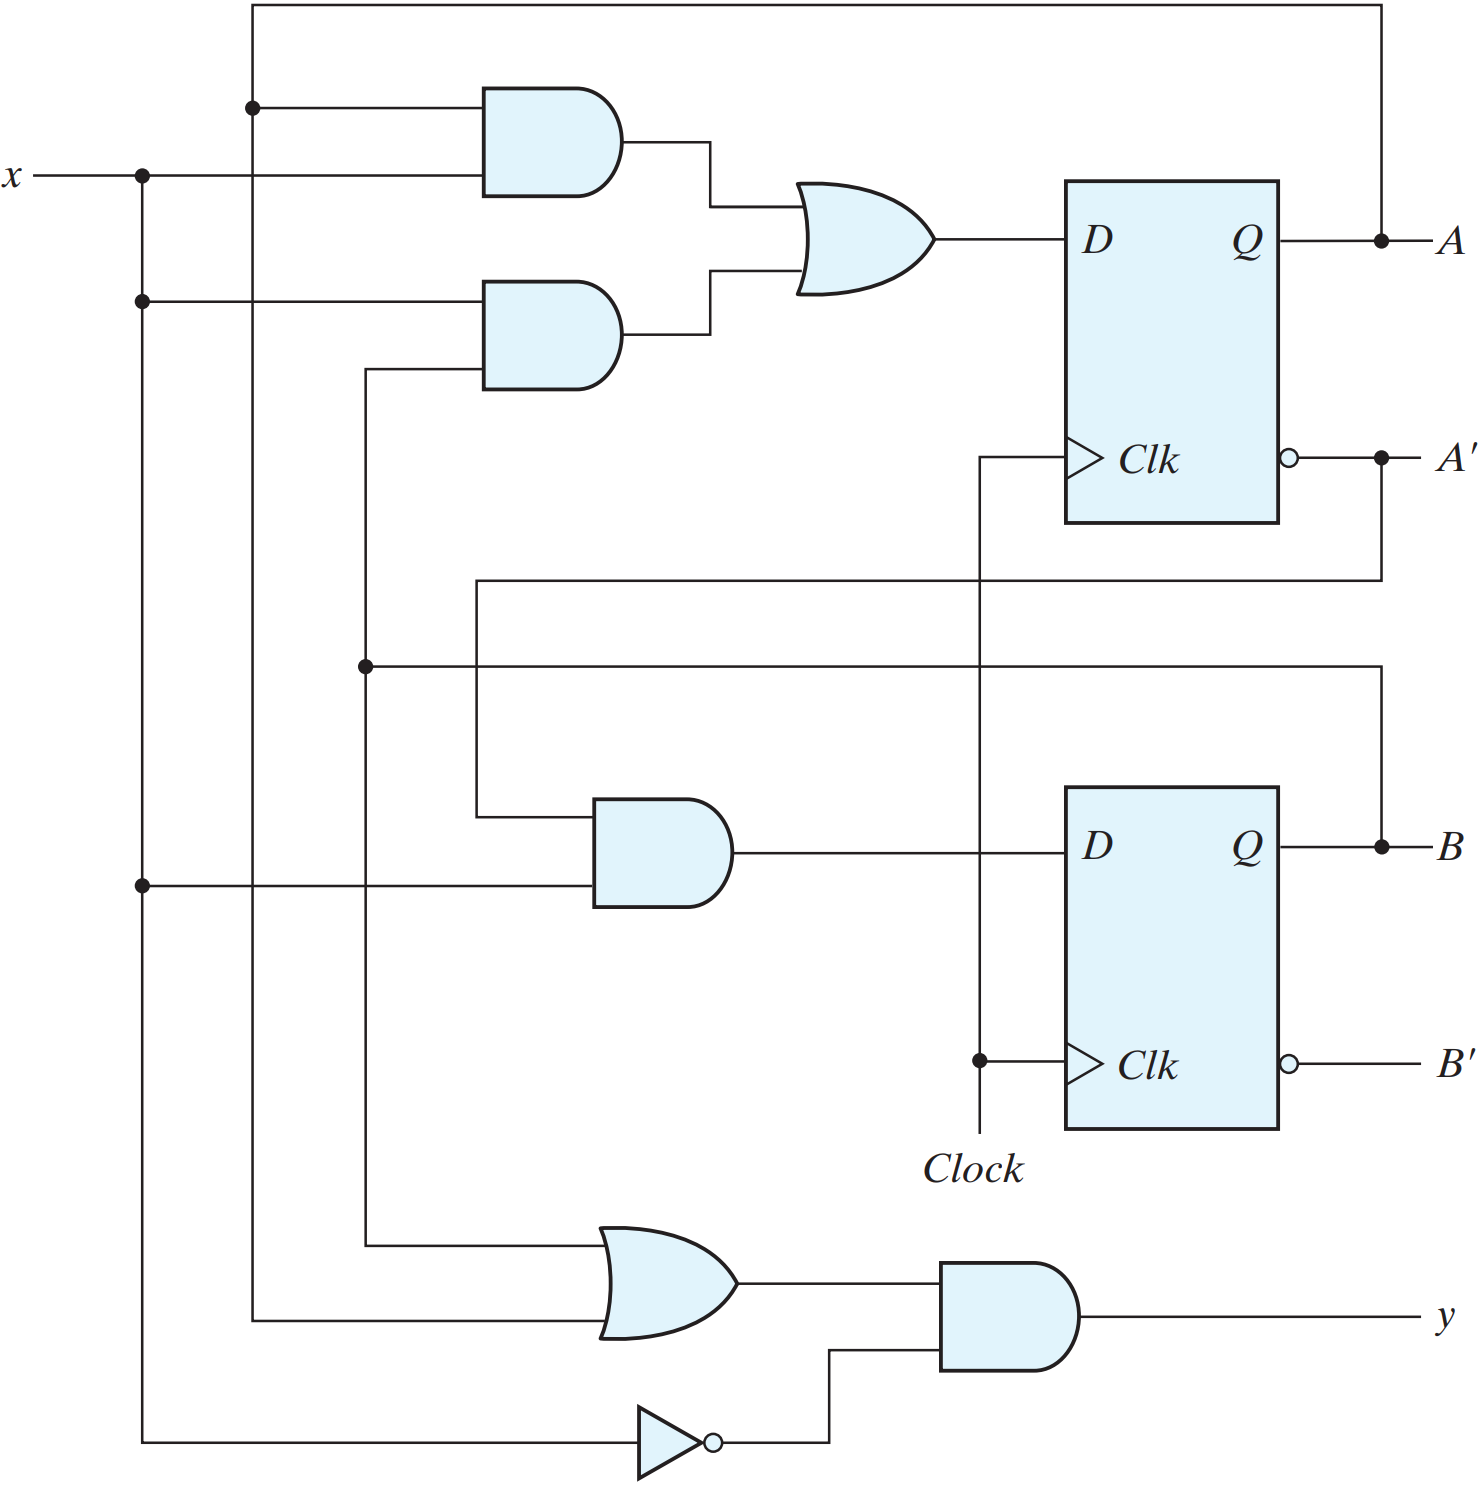
\includegraphics[width=\linewidth]{img/fig-5.15.png}
  \caption{Example of sequential circuit}
  \label{fig:5.15}
\end{figure}
\noindent So the state equations:
\begin{align*}
  A(t + 1) &= Ax + Bx\\
  B(t + 1) &= A'x\\
  y &= (A + B)x'
\end{align*}

\subsection{State Table}
\label{subsec:state-table}

The time sequence of inputs, outputs, and flip-flop states can be enumerated in a \textit{state table} (sometimes called a \textit{transition table}). The state table for the circuit of Fig. 15 is shown in Table 5.2. The table consists of four sections labeled \textit{present state}, \textit{input}, \textit{next state}, and \textit{output}.

\noindent The derivation of a state table requires listing all possible binary combinations of present states and inputs. In general, a sequential circuit with $m$ flip-flops and $n$ inputs needs $2^{m + n}$ rows in the state table.

\vspace*{\fill}
\columnbreak

\begin{figure}[H]
  \centering
  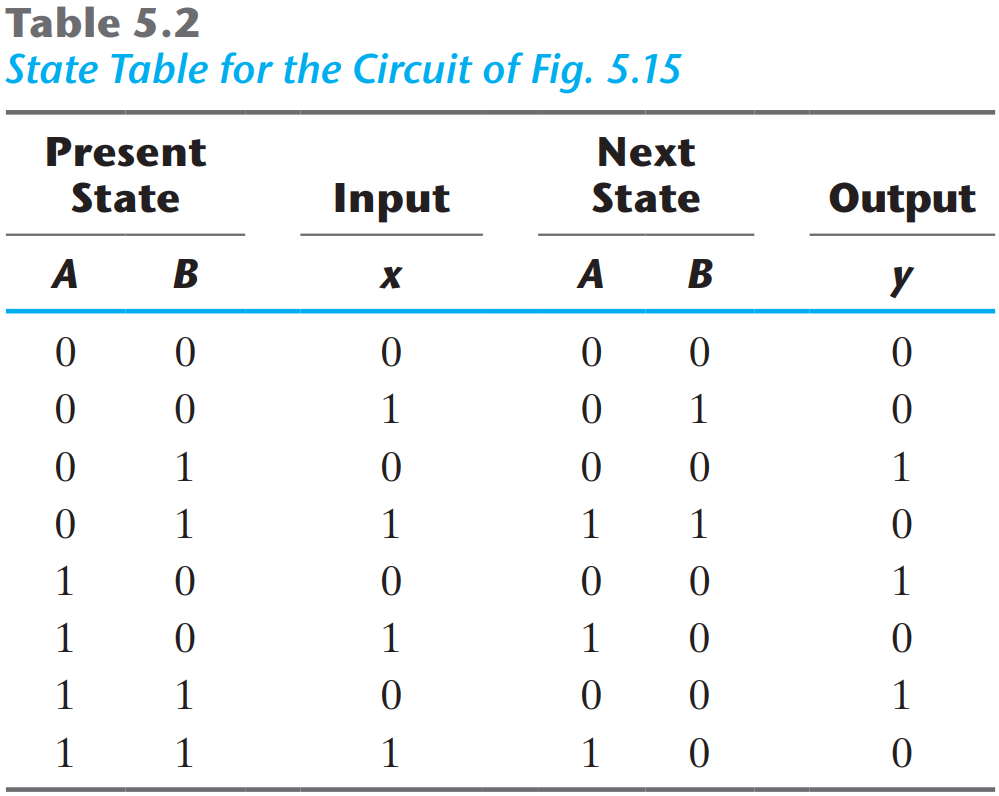
\includegraphics[width=.8\linewidth]{img/table-5.2.png}
  \label{table:5.2}
\end{figure}

It is sometimes convenient to express the state table in a slightly different form having only three sections: \textit{present state}, \textit{next state}, and \textit{output}. The input conditions are enumerated under the next-state and output sections. The state table of Table 5.2 is  repeated in Table 5.3 in this second form.
\begin{figure}[H]
  \centering
  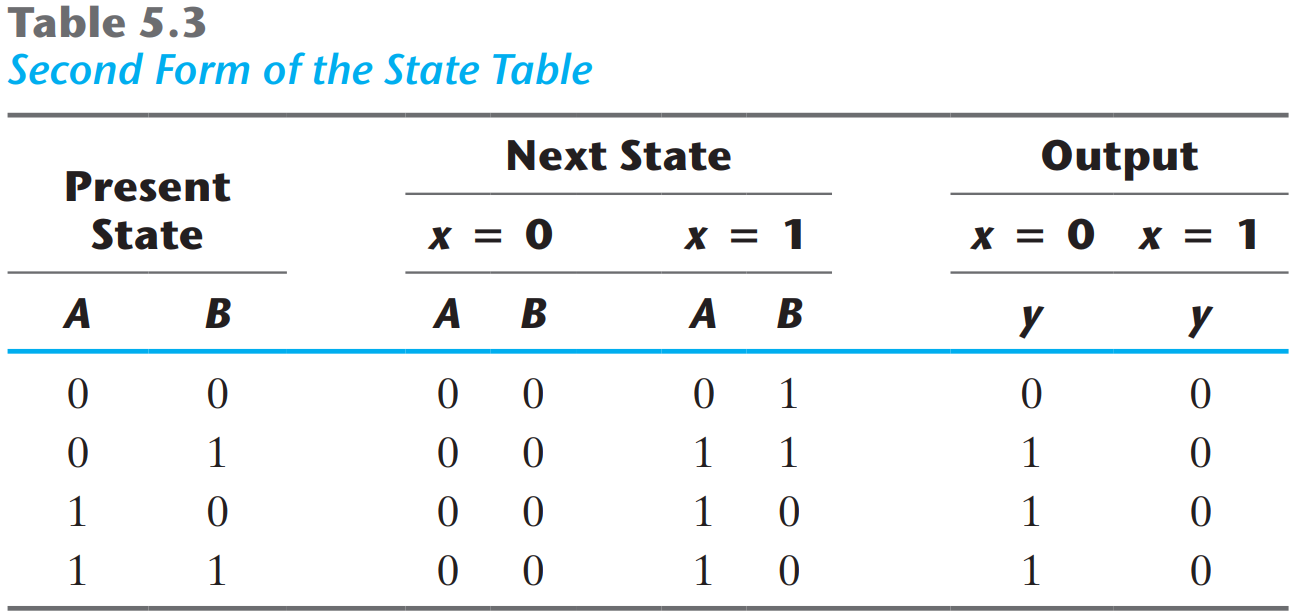
\includegraphics[width=.9\linewidth]{img/table-5.3.png}
  \label{table:5.3}
\end{figure}

\subsection{State Diagram}
\label{subsec:state-diagram}

The information available in a state table can be represented graphically in the form of a state diagram. In this type of diagram, a state is represented by a circle, and the (clock-triggered) transitions between states are indicated by directed lines connecting the circles.

The state diagram of the sequential circuit of Fig. 15 is shown in Fig. 16. The state diagram provides the same information as the state table and is obtained directly from Table 5.2 or Table 5.3. The binary number inside each circle identifies the state of the flip-flops. The directed lines are labeled with two binary numbers separated by a slash. The input value during the present state is labeled first, and the number after the slash gives the output during the \textit{present} state with the given input.
\begin{figure}[H]
  \centering
  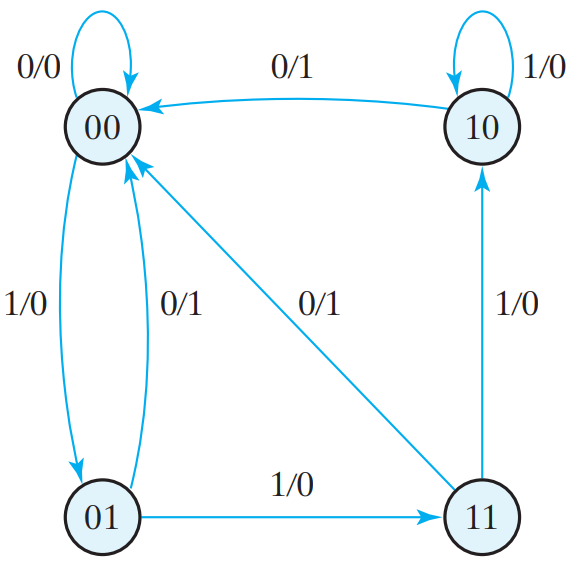
\includegraphics[width=.5\linewidth]{img/fig-5.16.png}
  \caption{State diagram of the circuit of Fig. 15}
  \label{fig:5.16}
\end{figure}

\noindent The steps presented in this example are summarized below:
\begin{center}
  Circuit diagram $\ra$ State Equations $\ra$ State Table $\ra$ State Diagram
\end{center}

\noindent To analyze sequential circuits:
\begin{itemize}
  \item Find Boolean expressions for the outputs of the circuit and the flip-flop inputs.
  \item Use these expressions to fill in the output and flip-flop input columns in the state table.
  \item Finally, use the characteristic equation or characteristic table of the flip-flop to fill in the next state columns.
\end{itemize}
The result of sequential circuit analysis is a state table or a state diagram describing the circuit.

\textit{\textbf{Note:} There are some examples in book that are realted to analysis. Examine them carefully.}

\subsection{Mealy and Moore Models of Finite State Machine}
\label{subsec:mealy-and-moore-models}

\begin{figure}[H]
  \centering
  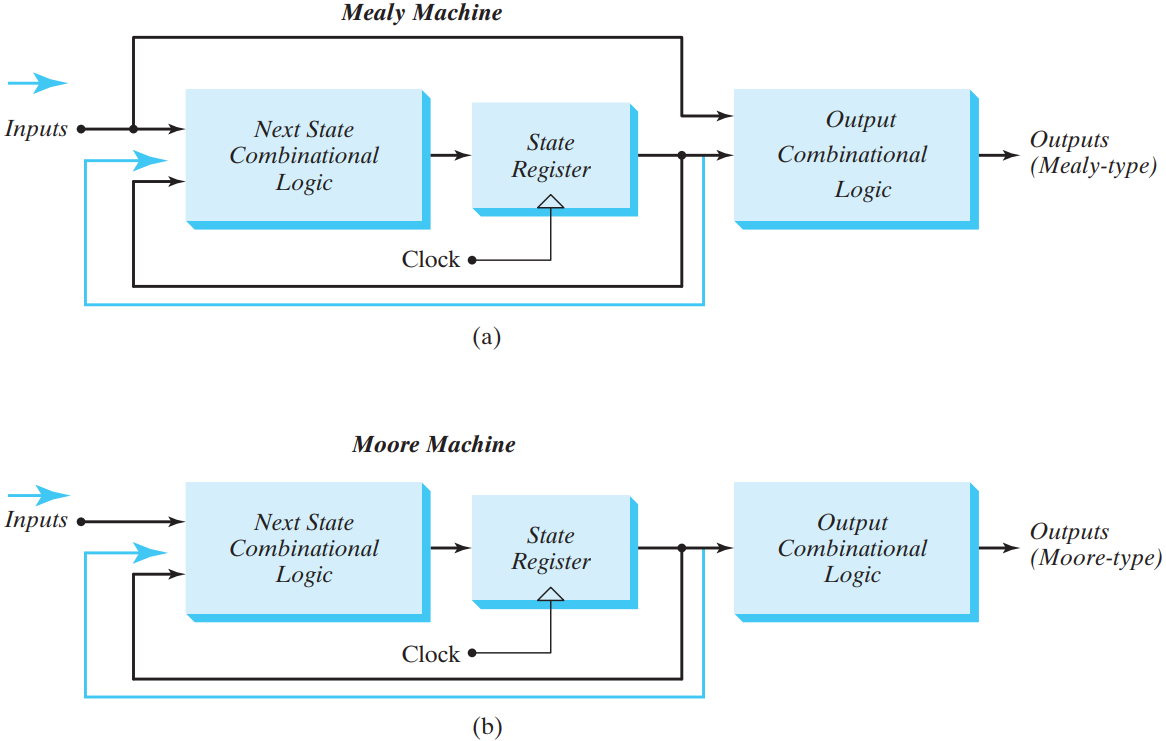
\includegraphics[width=\linewidth]{img/fig-5.21.png}
  \caption{}
  \label{fig:5.21}
\end{figure}

In a Moore model, the outputs of the sequential circuit are synchronized with the  clock, because they depend only on flip-flop outputs, which are synchronized with the clock.

The output of the Mealy machine is the value that is present immediately before the active edge of the clock.

\textbf{Notes:}
\begin{itemize}
  \item The difference between a Mealy and Moore state machine is that ``\textit{the output of a Moore state machine depends on only the state of the machine; the output of a Mealy machine depends on the present state and the inputs to the machine.}
  \item \textit{The edge of a state machine chart represents a transition of the machine between two states.}
  \item \textit{A transition between the states of a finite state machine occurs at the active edge of the synchronizing signal (clock).}
  \item \textit{A finite state machine may have synchronous or asynchronous reset.}
  \item The reason why it is an important practice to implement a reset  signal in a finite state machine is that ``\textit{ Without a reset signal a finite state machine cannot be driven into a known initial state.}''.
  \item \textit{The outputs of a Mealy state machine may depend on the inputs to the machine.}
\end{itemize}